\documentclass{article}

\usepackage[margin=0.75in]{geometry}
\usepackage{amsmath,amsthm,amssymb}
\usepackage{graphicx,float}
\usepackage{multirow,setspace}
\usepackage{natbib,enumerate}
\usepackage{caption}
\usepackage{subcaption}
\usepackage{termcal} 
\usepackage{xcolor}
\usepackage{enumitem}
\usepackage{gensymb}
\usepackage{multicol}
\usepackage{listings}
\usepackage{booktabs}


\setlength{\marginparwidth}{2cm}

\renewcommand{\thesection}{\Alph{section}}
\newcommand{\HRule}{\rule{\linewidth}{0.5mm}}
\newcommand{\tab}{\hspace{0.5cm}}
\newcommand{\modref}[1]{(\ref{#1})}

\newcommand{\bbeta}{{\mbox{\boldmath$\beta$}}}
\newcommand{\bmu}{{\mbox{\boldmath$\mu$}}}
\newcommand{\balpha}{{\mbox{\boldmath$\alpha$}}}
\newcommand{\btheta}{{\mbox{\boldmath$\theta$}}}
\newcommand{\bpi}{{\mbox{\boldmath$\pi$}}}
\newcommand{\R}{\texttt{R}}
\newcommand{\Lik}{\mathcal{L}}

\begin{document}

%%% HEADER %%%
	\begin{center}
		\HRule \\[0.1cm]
		\vspace{0.1cm}
		{ \LARGE \bfseries MATH 2625: Biostatistical Methods\\[0.5cm] Homework 5, due Thursday, April 10 } \\[0.1cm]
		\HRule \\[0.1cm]
	\end{center}
	
		Please submit a PDF or .doc version of your homework to Canvas by 3:30pm on the due date. Please type \emph{all} responses. You are encouraged to use \R\ for all calculations.
		
	\section*{Theory}
	\begin{enumerate}
		\item Find the estimated parametric survivor, hazard, and cumulative hazard functions for each of the following distributions. Because these distributions require root finding algorithms to find the MLE for some of their parameters, we will fix those parameters at the values specified below. Please show all of your work.
		\begin{enumerate}
			\item $T_i \sim Pa(\mu, \alpha)$ for $i = 1, \ldots, n$, $\mu = T_{(1)}$ (i.e. the minimum survival time), and $\alpha$ unknown.
			\item $T_i \sim W(\lambda, \gamma)$  for $i = 1, \ldots, n$, $\gamma = 2$, and $\lambda$ unknown.
		\end{enumerate}
	\end{enumerate}

	\begin{proof}
	The pdf of $T_i \sim Pa(\mu, \alpha)$ is defined as

	\[ f(t) = \frac{\alpha\mu^\alpha}{t^{\alpha + 1}}.\] % pareto distribution PDF

	We can integrate $f(t)$ to find the cdf, $F(t)$.

	\begin{align*}
		F(t) = \int f(t)dt & = \int\frac{\alpha\mu^\alpha}{t^{\alpha + 1}} dt \\
		& = \alpha\mu^\alpha \left( \frac{1}{\alpha t^{\alpha}} \right) \\
		& = \left( \frac{\mu}{t} \right)^\alpha .
	\end{align*} % pareto distribution CDF (line above)

	Then our survival function $S(t)$ is defined as

	\[S(t) = 1 - \left( \frac{\mu}{t} \right)^\alpha .\] % survival function here!!!

	The hazard function $h(t)$ of the Pareto distribution is then
	
	\[h(t) = \frac{ \frac{\alpha\mu^\alpha}{t^{\alpha + 1}} }{ \left( \frac{\mu}{t}\right) ^\alpha } .\]

	This simplifies to

	\[ h(t) = \frac{\alpha}{t}.\]

	
	Now we will use the method of maximum likelihood to estimate $\hat{\alpha}$. The likelihood function of the Pareto distribtuion is

	\[L(t) = \prod_{i = 1}^{i = n} \frac{\alpha\mu^\alpha}{t^{\alpha + 1}}\]

	The log-likelihood of this function is

	\[ \]


	\end{proof}

	\newpage
	\section*{Case Studies}
	For each of the following case studies, create a structured abstract no longer than 4 pages in length (including figures, tables, and references). The Background section is provided for each and should be included in your write-up. You must write the Methods, Results, and Conclusion sections. Code should be included in an appendix as well.

	\begin{enumerate}
		\item The first Case Study looks at bladder cancer, both its recurrence and death due to bladder cancer. The data can be found in the file \texttt{bladder.txt}. Variables include subject's \texttt{id}, \texttt{time} (to recurrence, death, or censored in months), first recurrence status (\texttt{status1}, coded 1 for first recurrence, 0 for censored or dead), death status (\texttt{status2}, coded 1 for dead, 0 for censored or first recurrence), \texttt{treatment} (code \texttt{placebo}, \texttt{pyridoxine}, and \texttt{thiotepa}), the \texttt{number} of initial \texttt{number} tumors (coded \texttt{One}, \texttt{Two or Three}, and \texttt{Four or More}), and the \texttt{size} of the largest tumor (coded \texttt{1cm}, \texttt{2cm to 3cm}, and \texttt{4cm or Larger}).
		
		\item The second Case Study examines the time to first and second recurrence of chronic granulomatous disease or CGD. As only a subset of the patients had the second recurrence, there are two datasets for this study: \texttt{cgd1.txt} (first recurrence data) and \texttt{cgd2.txt} (second recurrence data). The variables in both datasets have the same names. Variables include subejct's \texttt{id}, the \texttt{time} to recurrence of infection in days, \texttt{status} (1 for recurrence, 0 for censored), \texttt{treatment} (coded \texttt{rIFN-g} for gamma r-interferon, \texttt{placebo}), pattern of inheritance (\texttt{inherit}, coded \texttt{autosomal} or \texttt{X-linked}), and use of prophylactic antibiotics at study entry (\texttt{propylac}, coded 1 for yes, 0 for no).

	\subsection*{Background}

	Chronic granulomatous disease or CGD is a genetic disorder in which white blood cells called phagocytes are unable to kill certain types of bacteria and fungi. Consequently, patients suffering from CGD are subject to frequent and potentially life-threatening infections. CGD impacts the effectiveness of phagocytes, a type of white blood cell, that makes patients more susceptible to bacterial and fungal infections. We conducted a placebo controlled trial of a cytokine-based treatment using interferon gamma to examine its effect on recurrence of CGD. The primary endpoint of the study was the first recurrence of a bacterial or fungal infection and the secondary endpoint was the second recurrence of infection. The pattern of inheritance and use of antibiotics may impact recurrence as well. In total, 128 patients were available for analysis of the primary endpoint while only 44 patients were available for the secondary endpoint.

		
	
	\end{enumerate}

	\newpage
	\subsection*{Background} % move these around to fix indent

	Bladder cancer is a common type of cancer, typically beginning in the urothelial cells of the bladder. The cancer is often caught in the early stages and is easily treatable. However, even early-stage surgical interventions may not prevent recurrence. To evaluate the effectiveness of post-surgical treatments, we conducted a three arm study comparing the effects of treatment with pyridoxine, thiotepa, or placebo on the primary end point of recurrence. We also consider the secondary end point of death. The size of the initial tumor or the number of initial tumors may also impact both study endpoints. We enrolled 118 patients with confirmed bladder cancer whose tumors were surgically removed and followed them until recurrence, death, or both.


	\subsection*{Methods}
	118 patients with bladder cancer whose tumors were removed via surgery were selected for this randomized controlled trial. The subjects were randomly given one of three treatments: pyridoxine, thiotepa, or a placebo. We followed patients after their treatment to determine whether patients had a recurrence of bladder cancer. We also examined whether or not the patients died. While there was a possibility of patients developing both outcomes of interest, we only observed the outcome that came first. The subject was subsequently considered censored for the other outcome.

	We used Kaplan-Meier estimation to estimate the survival functions of recurrence of cancer as well as death for each of the three treatment groups. Estimates of the median time to tumor recurrence and death were also found when available. We used a Gehan-Breslow-Wilcoxon Test to determine whether there was a significant difference in the survival curves for both outcomes over time in subjects with each of the different treatments. We also used Kaplan-Meier estimation to conduct secondary analyses on the interaction on the time to cancer recurrence of two potential confounders: size of a subject’s initial tumor and the number of initial tumors in a subject. All analyses were done at the nominal level.

	\subsection*{Results}
	Among the 118 patients who were selected for the study, 32 received pyridoxine, 38 received thiotepa, and the remaining 48 formed the placebo control group. 17 of the subjects died under study observation, and 62 had a recurrence of bladder cancer. We observed the longest median time to cancer recurrence in patients receiving pyridoxine of 42 months. We did not observe a median survival time for patients receiving pyridoxine or the placebo, as the death counts in these two treatment arms were very low. However, with censored subjects taken into account, we estimated a median survival time for patients receiving thiotepa to be 59 months.

	% TABLE ONE
	\begin{table}[ht]
		\centering
		\footnotesize
		\caption*{\textbf{Table 1. Time to Cancer Recurrence \& Death of Patients by Treatment Group}}
		\begin{tabular}{@{}l l | l l | l l @{}}
			\toprule
			Treatment & \parbox[t]{2cm}{Number of\\ Patients} & \parbox[t]{2.5cm}{Observed\\ Recurrences} & \parbox[t]{3cm}{Median Time to\\ Recurrence (months)} & \parbox[t]{2.5cm}{Observed\\ Deaths} & \parbox[t]{3cm}{Median Time to\\ Death (months)} \\
			\midrule
			Pyridoxine & 32 & 15 & 42 & 6 & NA \\
			Thiotepa   & 38 & 18 & 26 & 6 & 59 \\
			Placebo    & 48 & 29 & 16 & 5 & NA \\
			\midrule
			Total      & 118 & 62 & & 17 & \\
			\bottomrule
		\end{tabular}
	\end{table}

	\begin{figure}[htbp]
		\centering
		\captionsetup{labelformat = empty}
		\begin{subfigure}[t]{0.32\textwidth}
			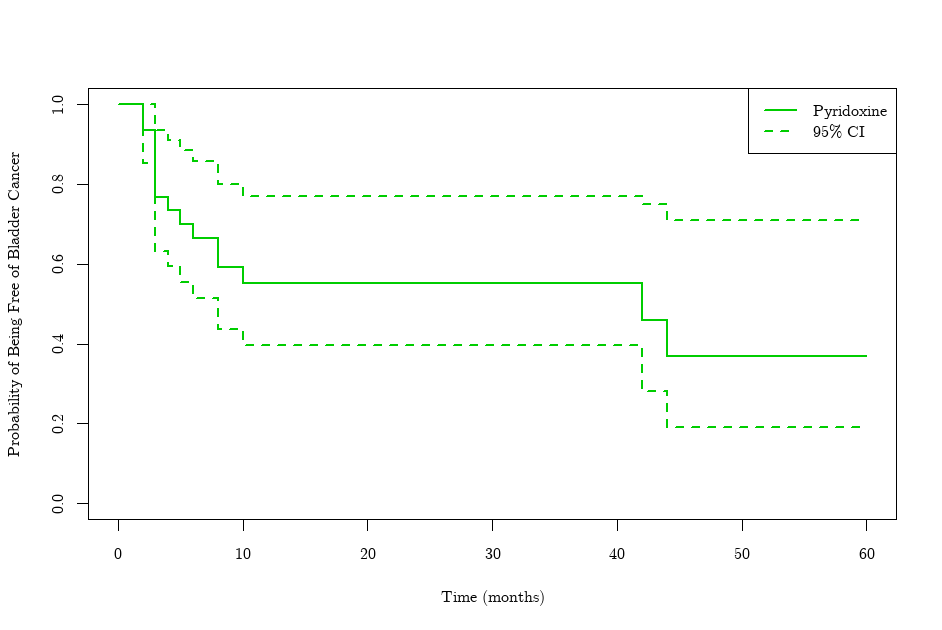
\includegraphics[width=\linewidth]{graphs/case1/recurrance~treatment_pyridoxine.png}
			\caption*{\raggedright\hyphenpenalty=10000\exhyphenpenalty=10000\sloppy 
			\textbf{Figure 1.} Time to Recurrence in Subjects Treated With Pyridoxine}
		\end{subfigure}
		\hfill
		\begin{subfigure}[t]{0.32\textwidth}
			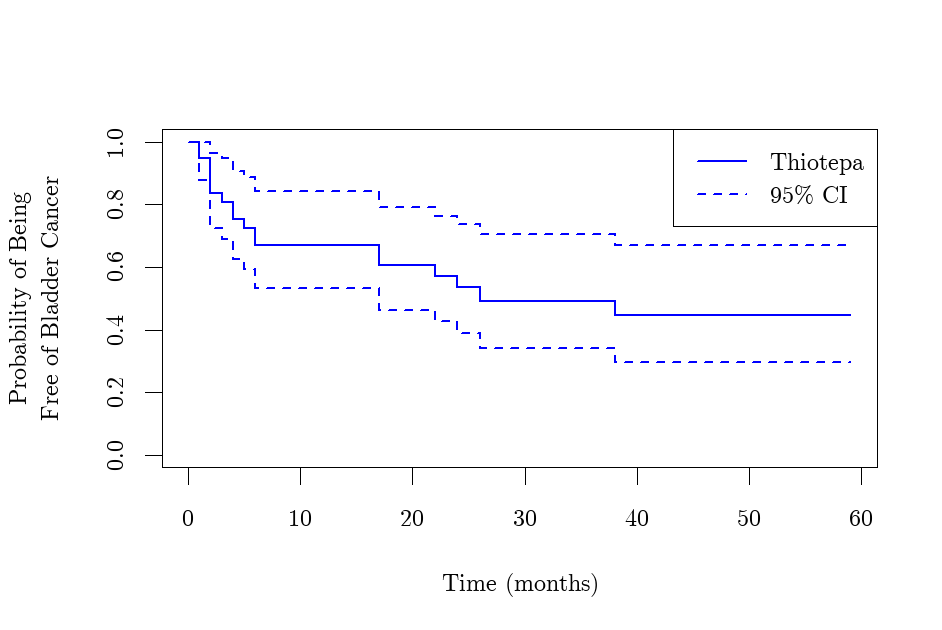
\includegraphics[width=\linewidth]{graphs/case1/recurrance~treatment_thiotepa.png}
			\caption*{\raggedright\hyphenpenalty=10000\exhyphenpenalty=10000\sloppy 
			\textbf{Figure 2.} Time to Recurrence in Subjects Treated With Thiotepa}
		\end{subfigure}
		\hfill
		\begin{subfigure}[t]{0.32\textwidth}
			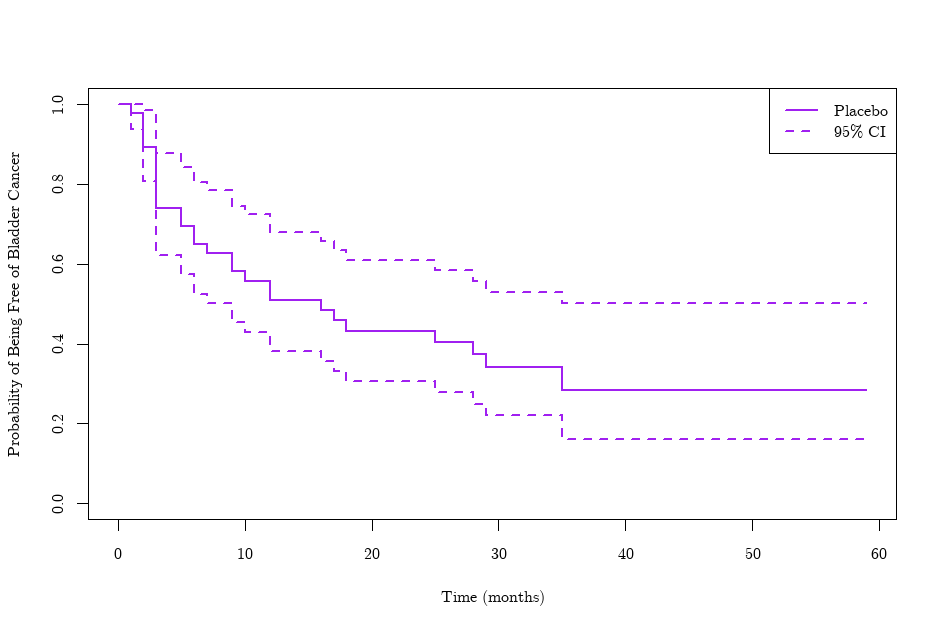
\includegraphics[width=\linewidth]{graphs/case1/recurrance~treatment_placebo.png}
			\caption*{\raggedright\hyphenpenalty=10000\exhyphenpenalty=10000\sloppy 
			\textbf{Figure 3.} Time to Recurrence in Control Group}
		\end{subfigure}
		\caption{Figures 1-3: Kaplan-Meier Estimates of Time to Bladder Cancer Recurrence for Each Treatment Group}
		\label{recur~treat_groups}
	  \end{figure} 
	  % Manually advance counter since we just "used" 3 figures
	  \addtocounter{figure}{2}
	  %%%%%%%%%%%%%%%%%%%%%%5

	% FIGURE FOUR: KAPLAN MEIER GRAPHS FOR ALL 3 TREATMENTS
	\begin{figure}[h!]
		\centering
		\tiny
		  \centering
		  \tiny
		  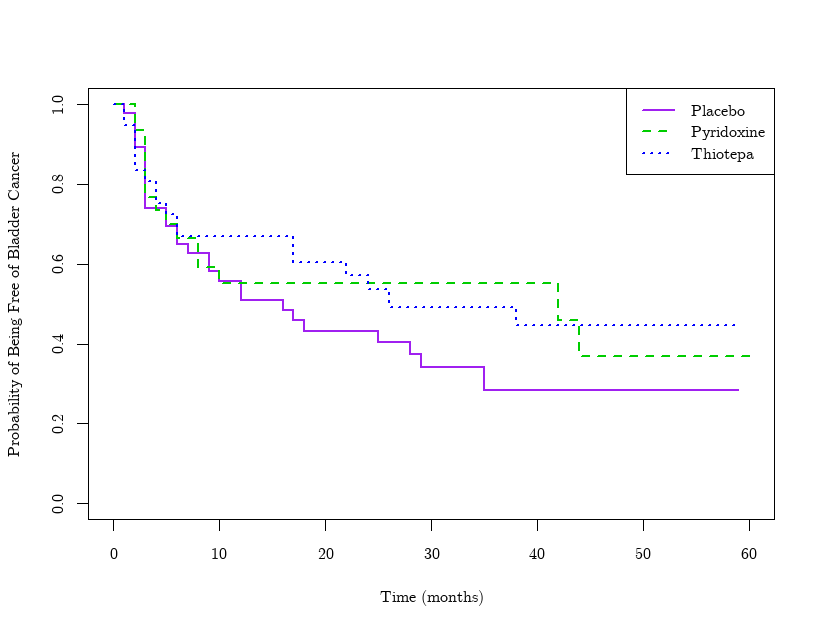
\includegraphics[width=0.6\textwidth]{graphs/case1/recurrance~treatment_all.png}
		  \caption{Kaplan-Meier Estimate of Time to Recurrence in Subjects by Treatment}
		  \label{recur~treat_all}
	\end{figure}

	  We did not find a statistically significant difference in recurrence rates over time between the three treatment groups $(p = 0.5, \chi^2 = 1.3$, df = 2). Figure 1 shows the Kaplan-Meier estimation of recurrence rates over time. We also did not find a significant difference in survival rates between the three treatment groups $(p = 0.8, \chi^2 = 0.5$, df = 2). Figure 5 shows Kaplan-Meier estimates of patient survival rates over time.

	  \begin{figure}[h!]
		\centering
		\tiny
		  \centering
		  \tiny
		  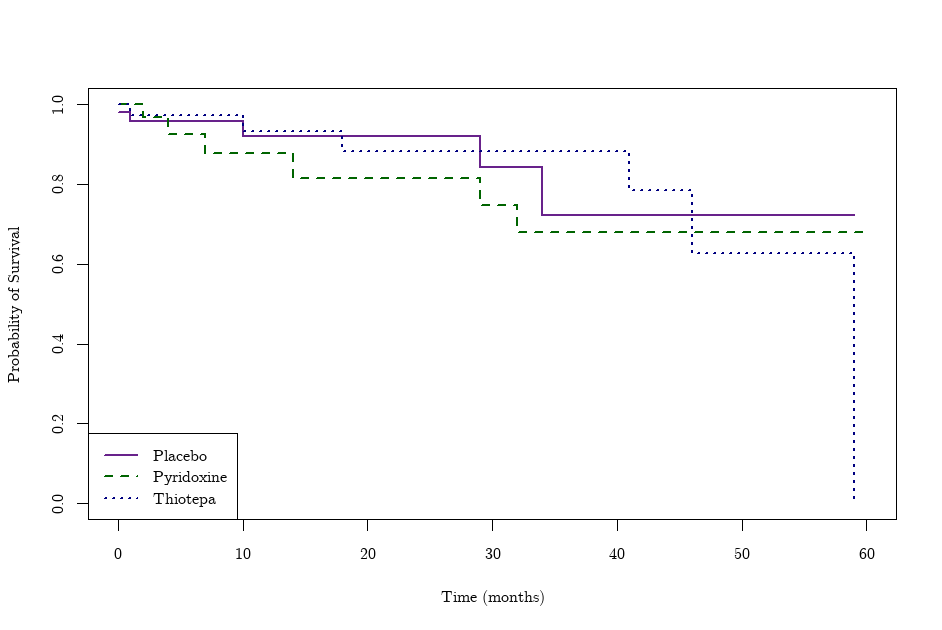
\includegraphics[width=0.6\textwidth]{graphs/case1/recurrance~death.png}
		  \caption{Kaplan-Meier Estimate of Survival Time in Subjects by Treatment}
		  \label{death~treat}
	\end{figure}

	\begin{table}[H]
		\centering
		\footnotesize
		\caption{\textbf{Time to Cancer Recurrence in Patients by Initial Number of Tumors}}
		\begin{tabular}{cccc}
			\toprule
			\multicolumn{1}{c}{Initial Number} & 
			\multicolumn{1}{c}{Number of} & 
			\multicolumn{1}{c}{Observed} & 
			\multicolumn{1}{c}{Median Time to} \\
			\multicolumn{1}{c}{of Tumors} & 
			\multicolumn{1}{c}{Patients} & 
			\multicolumn{1}{c}{Recurrences} & 
			\multicolumn{1}{c}{Recurrence (months)} \\
			\midrule
			One            & 72  & 30 & 42 \\
			Two to Three   & 27  & 17 & 24 \\
			Four or More   & 19  & 15 & 5  \\
			\midrule
			Total          & 118 & 62 &  \\
			\bottomrule
		\end{tabular}
	\end{table}

	\begin{table}[H]
		\centering
		\footnotesize
		\caption{\textbf{Time to Cancer Recurrence in Patients by Initial Size of Tumors}}
		\begin{tabular}{cccc}
			\toprule
			\multicolumn{1}{c}{Initial Size} & 
			\multicolumn{1}{c}{Number of} & 
			\multicolumn{1}{c}{Observed} & 
			\multicolumn{1}{c}{Median Time to} \\
			\multicolumn{1}{c}{of Tumors} & 
			\multicolumn{1}{c}{Patients} & 
			\multicolumn{1}{c}{Recurrences} & 
			\multicolumn{1}{c}{Recurrence (months)} \\
			\midrule
			1cm             & 69  & 38 & 22 \\
			2cm to 3cm      & 33  & 13 & N/A \\
			4cm or Larger   & 16  & 11 & 6  \\
			\midrule
			Total           & 118 & 62 &    \\
			\bottomrule
		\end{tabular}
	\end{table}


	%%%%%%%%%%%%%%% FIGURES FOR TUMOR SIZE AND COUNT
	\begin{figure}[htbp]
		\centering
		\captionsetup{labelformat = empty}
		\begin{subfigure}[t]{0.48\textwidth}
		  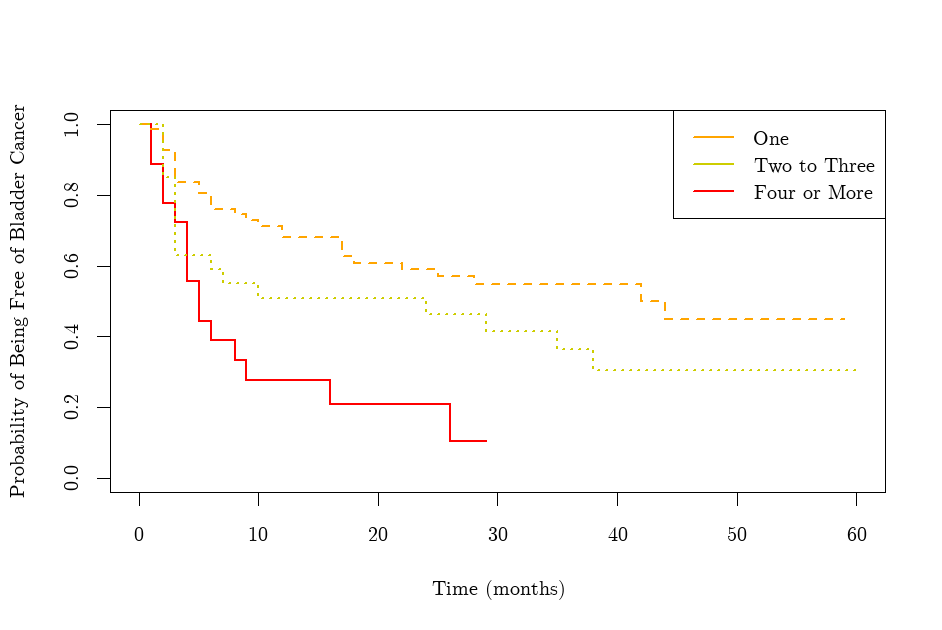
\includegraphics[width=\linewidth]{graphs/case1/recurrance~tumor_count.png}
		  \caption{Caption for the first image}
		  \label{surv-tumor-count}
		\end{subfigure}
		\hfill
		\begin{subfigure}[t]{0.48\textwidth}
		  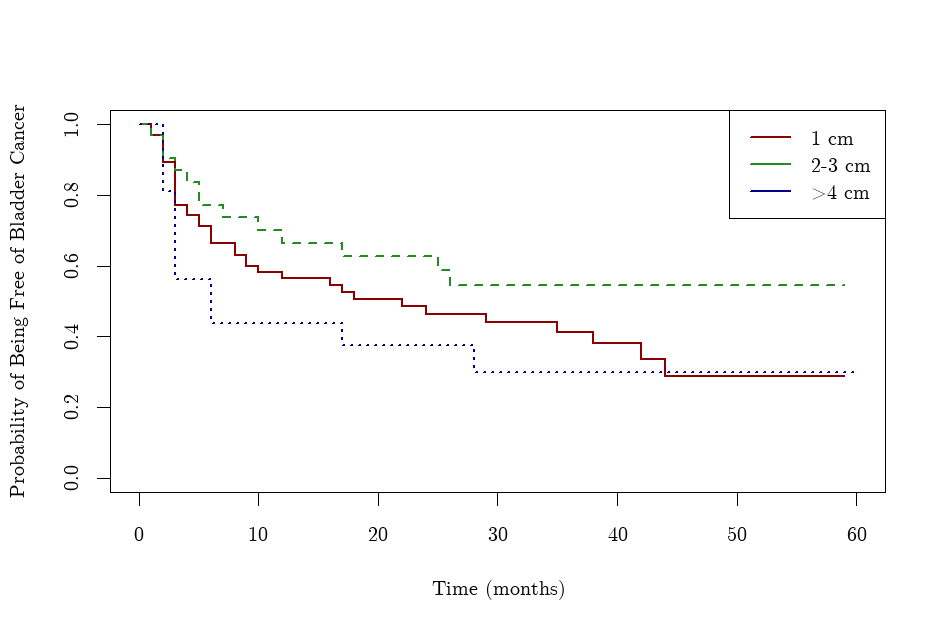
\includegraphics[width=\linewidth]{graphs/case1/recurrance~tumor_size.png}
		  \caption{Caption for the second image}
		  \label{surv-tumor-size}
		\end{subfigure}
		\caption{Figures 6-7: Kaplan-Meier Estimates of Time to Bladder Cancer by Number \& Size of Initial Tumors}
		\label{fig-confounders}
	  \end{figure}
	  \addtocounter{figure}{2}

	While 72 of the 118 subjects only had one prior tumor present, 19 had at least four tumors. Additionally, most tumors were within 1cm in size, while only 16 patients had tumors larger than 4cm in size. Tables 2 and 3 provide a more detailed break-down of the findings. There was a statistically significant difference in time to recurrence of cancer based on the initial number of tumors in a subject $(p < 0.001, \chi^2 = 13.9$, df = 2). We found that the time to the recurrence of cancer in a subject was lowest if the subject only had one tumor removed at the start of the study, as shown in Figure 6. However, we did not find evidence to suggest that the size of a subject’s initial tumor had an impact on the time to the recurrence of cancer $(p = 0.2, \chi^2 = 3.7$, df = 2).


	\subsection*{Discussion}
		
\end{document}














